%%%%%%%%%%%%%%%%%%%%%%%%%%%%%%%%%%%%%%%%%%%%%%%%%%%%%%%%%%%%%%%%%%%%%%%%%%%%
% AGUtmpl.tex: this template file is for articles formatted with LaTeX2e,
% Modified December 2018
%
% This template includes commands and instructions
% given in the order necessary to produce a final output that will
% satisfy AGU requirements.
%
% FOR FIGURES, DO NOT USE \psfrag
%
%%%%%%%%%%%%%%%%%%%%%%%%%%%%%%%%%%%%%%%%%%%%%%%%%%%%%%%%%%%%%%%%%%%%%%%%%%%%
%
% IMPORTANT NOTE:
%
% SUPPORTING INFORMATION DOCUMENTATION IS NOT COPYEDITED BEFORE PUBLICATION.
%
%
%
%%%%%%%%%%%%%%%%%%%%%%%%%%%%%%%%%%%%%%%%%%%%%%%%%%%%%%%%%%%%%%%%%%%%%%%%%%%%
%
% Step 1: Set the \documentclass
%
%
% PLEASE USE THE DRAFT OPTION TO SUBMIT YOUR PAPERS.
% The draft option produces double spaced output.
%
% Choose the journal abbreviation for the journal you are
% submitting to:

% jgrga JOURNAL OF GEOPHYSICAL RESEARCH (use for all of them)
% gbc   GLOBAL BIOCHEMICAL CYCLES
% grl   GEOPHYSICAL RESEARCH LETTERS
% pal   PALEOCEANOGRAPHY
% ras   RADIO SCIENCE
% rog   REVIEWS OF GEOPHYSICS
% tec   TECTONICS
% wrr   WATER RESOURCES RESEARCH
% gc    GEOCHEMISTRY, GEOPHYSICS, GEOSYSTEMS
% sw    SPACE WEATHER
% ms    JAMES
% ef    EARTH'S FUTURE
%
%
%
% (If you are submitting to a journal other than jgrga,
% substitute the initials of the journal for "jgrga" below.)

\documentclass[ef,draft]{agutexSI2019}

% fonts and appearance
\usepackage{amsmath, amsfonts, physics, siunitx, nicefrac}

% better tables
\usepackage{booktabs}
\usepackage{array}
\newcommand{\PreserveBackslash}[1]{\let\temp=\\#1\let\\=\temp}
\newcolumntype{C}[1]{>{\PreserveBackslash\centering}p{#1}}
\newcolumntype{R}[1]{>{\PreserveBackslash\raggedleft}p{#1}}
\newcolumntype{L}[1]{>{\PreserveBackslash\raggedright}p{#1}}

\usepackage{xspace}
\makeatletter
\DeclareRobustCommand\onedot{\futurelet\@let@token\@onedot}
\def\@onedot{\ifx\@let@token.\else.\null\fi\xspace}
\def\eg{\emph{e.g}\onedot} \def\Eg{\emph{E.g}\onedot}
\def\ie{\emph{i.e}\onedot} \def\Ie{\emph{I.e}\onedot}
\def\etc{\emph{etc}\onedot} \def\vs{\emph{vs}\onedot}
\newcommand{\usd}[1]{\SI{#1}[\$]{}}

% ACRONYMS
\usepackage[acronym, nopostdot, nonumberlist, shortcuts, numberedsection, nogroupskip,]{glossaries}
\newacronym{bfe}{BFE}{base flood elevation}
\newacronym{cmip}{CMIP}{the Coupled Model Intercomparison Project}
\newacronym{dmdu}{DMDU}{decision making under deep uncertainty}
\newacronym{fema}{FEMA}{the Federal Emergency Management Agency}
\newacronym{gev}{GEV}{generalized extreme value}
\newacronym{hazus}{HAZUS}{Hazard U.S.}
\newacronym{iid}{IID}{independent and identically distributed}
\newacronym{ipcc}{IPCC}{International Panel on Climate Change}
\newacronym{msl}{MSL}{mean relative sea level}
\newacronym{noaa}{NOAA}{the National Oceanic and Atmospheric Administration}
\newacronym{pdf}{PDF}{probability density function}
\newacronym{rcp}{RCP}{representative concentration pathway}
\newacronym{rdm}{RDM}{robust decision making}
\newacronym{slr}{SLR}{sea level rise}
\newacronym{ssp}{SSP}{shared socio-economic pathway}
\newacronym[]{usace}{USACE}{United States Army Corps of Engineers}
\newacronym[]{usgs}{USGS}{United States Geological Survey}
\newacronym[plural=SOWs,firstplural=states of the world (SOWs),descriptionplural=states of the world]{sow}{SOW}{state of the world}

%%%%%%%%%%%%%%%%%%%%%%%%%%%%%%%%%%%%%%%%%%%%%%%%%%%%%%%%%%%%%%%%%%%%%%%%%
%
%  SUPPORTING INFORMATION TEMPLATE
%
%% ------------------------------------------------------------------------ %%
%
%
%Please use this template when formatting and submitting your Supporting Information.

%This template serves as both a “table of contents” for the supporting information for your article and as a summary of files.
%
%
%OVERVIEW
%
%Please note that all supporting information will be peer reviewed with your manuscript. It will not be copyedited if the paper is accepted.
%In general, the purpose of the supporting information is to enable authors to provide and archive auxiliary information such as data tables, method information, figures, video, or computer software, in digital formats so that other scientists can use it.
%The key criteria are that the data:
% 1. supplement the main scientific conclusions of the paper but are not essential to the conclusions (with the exception of
%    including %data so the experiment can be reproducible);
% 2. are likely to be usable or used by other scientists working in the field;
% 3. are described with sufficient precision that other scientists can understand them, and
% 4. are not exe files.
%
%USING THIS TEMPLATE
%
%***All references should be included in the reference list of the main paper so that they can be indexed, linked, and counted as citations.  The reference section does not count toward length limits.
%
%All Supporting text and figures should be included in this document. Insert supporting information content into each appropriate section of the template. To add additional captions, simply copy and paste each sample as needed.

%Tables may be included, but can also be uploaded separately, especially if they are larger than 1 page, or if necessary for retaining table formatting. Data sets, large tables, movie files, and audio files should be uploaded separately. Include their captions in this document and list the file name with the caption. You will be prompted to upload these files on the Upload Files tab during the submission process, using file type “Supporting Information (SI)”

%IMPORTANT NOTE ON FIGURES AND TABLES
% Placeholders for figures and tables appear after the \end{article} command, after references.
% DO NOT USE \psfrag or \subfigure commands.
%
 \usepackage{graphicx}
 \graphicspath{{../../plots/}{../../tikz/}{../../img/}}
%
%  Uncomment the following command to allow illustrations to print
%   when using Draft:
\setkeys{Gin}{draft=false}
%
% You may need to use one of these options for graphicx depending on the driver program you are using. 
%
% [xdvi], [dvipdf], [dvipsone], [dviwindo], [emtex], [dviwin],
% [pctexps],  [pctexwin],  [pctexhp],  [pctex32], [truetex], [tcidvi],
% [oztex], [textures]
%
%
%% ------------------------------------------------------------------------ %%
%
%  ENTER PREAMBLE
%
%% ------------------------------------------------------------------------ %%

% Author names in capital letters:
\authorrunninghead{DOSS-GOLLIN AND KELLER}

% Shorter version of title entered in capital letters:
\titlerunninghead{Synthesizing Deep Uncertainties}

%Corresponding author mailing address and e-mail address:
\authoraddr{Corresponding author: J. Doss-Gollin, Department of Civil and Environmental Engineering, Rice University, Houston, TX, USA (jdossgollin@rice.edu)}



% cite things in supplemental info file
\usepackage{xr}
\externaldocument{submission_02}

% this goes last
\usepackage{cleveref}
\begin{document}

%% ------------------------------------------------------------------------ %%
%
%  TITLE
%
%% ------------------------------------------------------------------------ %%

%\includegraphics{agu_pubart-white_reduced.eps}


\title{Supporting Information for ``A subjective Bayesian framework for synthesizing deep uncertainties in climate risk management''}
%
% e.g., \title{Supporting Information for "Terrestrial ring current:
% Origin, formation, and decay $\alpha\beta\Gamma\Delta$"}
%
%DOI: 10.1002/%insert paper number here%

%% ------------------------------------------------------------------------ %%
%
%  AUTHORS AND AFFILIATIONS
%
%% ------------------------------------------------------------------------ %%


% List authors by first name or initial followed by last name and
% separated by commas. Use \affil{} to number affiliations, and
% \thanks{} for author notes.
% Additional author notes should be indicated with \thanks{} (for
% example, for current addresses).

% Example: \authors{A. B. Author\affil{1}\thanks{Current address, Antartica}, B. C. Author\affil{2,3}, and D. E.
% Author\affil{3,4}\thanks{Also funded by Monsanto.}}

\authors{James Doss-Gollin\affil{1}, Klaus Keller\affil{2}}
\affiliation{1}{Department of Civil and Environmental Engineering, Rice University}
\affiliation{2}{Thayer School of Engineering, Dartmouth College}





%% ------------------------------------------------------------------------ %%
%
%  BEGIN ARTICLE
%
%% ------------------------------------------------------------------------ %%

% The body of the article must start with a \begin{article} command
%
% \end{article} must follow the references section, before the figures
%  and tables.

\begin{article}

      This document contains supplementary methods, figures, and tables for the paper ``A subjective Bayesian framework for synthesizing deep uncertainties in climate risk management'' by James Doss-Gollin and Klaus Keller.

      % Add an S to figures, tables, and sections
      \newcommand{\hbAppendixPrefix}{S}
      \renewcommand{\thesection}{\hbAppendixPrefix \arabic{section}}
      \renewcommand{\thefigure}{\hbAppendixPrefix\arabic{figure}}
      \setcounter{figure}{0}
      \renewcommand{\thetable}{\hbAppendixPrefix\arabic{table}}
      \setcounter{table}{0}
      \renewcommand{\theequation}{\hbAppendixPrefix\arabic{equation}}
      \setcounter{equation}{0}

      \section{Supplemental methods}

      \subsection{Statistical distributions}

      To avoid ambiguity, we define here some statistical distributions used in the main text.
      Except where otherwise indicated, we follow the default notation of the Distributions.jl Julia package \cite{besancon_distributions.jl:2021}.

      \subsubsection{Generalized Extreme Value distribution}
      We parameterize the \gls{gev} distribution as
      \begin{equation}\label{eq:gev-dist}
            f(x | \mu, \sigma, \xi)= \begin{cases}
                  \frac{1}{\sigma} \qty[ 1 + \qty( \frac{x-\mu}{\sigma} ) \xi ]^{-1 / \xi - 1} \exp \qty{- \qty[1+\qty(\frac{x-\mu}{\sigma}) \xi ]^{-1 / \xi} }, & \xi \neq 0 \\
                  \frac{1}{\sigma} \exp \qty{-\frac{x-\mu}{\sigma}} \exp \qty{ -\exp \qty[-\frac{x-\mu}{\sigma}]},                                               & \xi=0.
            \end{cases}
      \end{equation}

      \subsubsection{Inverse Gamma distribution}
      Parameterizing the Inverse Gamma distribution as
      \begin{equation}\label{eq:inv-gamma-dist}
            f(x | \alpha, \theta) = \frac{\theta^\alpha x^{-(\alpha + 1)}}{\Gamma(\alpha)} e^{-\frac{\theta}{x}}, \quad x > 0,
      \end{equation}
      the parameters $\alpha$ and $\theta$ can be computed from the desired mean $\mu$ and standard deviation $\sigma$ as
      \begin{align}\label{eq:inv-gamma-params}
            \begin{split}
                  \alpha &= 2 + \frac{\mu^2}{\sigma^2} \\
                  \theta &= \mu \qty(\alpha - 1).
            \end{split}
      \end{align}

      \subsubsection{Gamma distribution}
      We parameterize the Gamma distribution as
      \begin{equation}\label{eq:gamma-dist}
            f(x | \alpha, \theta) = \frac{x^{\alpha-1} e^{-x/\theta}}{\Gamma(\alpha) \theta^\alpha},
            \quad x > 0.
      \end{equation}

      \subsubsection{Plotting position}
      The plotting position used in \cref{fig:surge-obs-return} is the Weibull (``empirical'') plotting position
      \begin{equation}\label{eq:weibull}
            \nicefrac{r}{N + 1}
      \end{equation}
      where $N$ is the sample size and $r$ is the order of the $N$ observations ($r=1$ is the largest, $r=N$ is the smallest).

      \subsection{Algorithm to estimate expected damages}\label{sec:alg-ead}

      As discussed in \cref{sec:case-metrics}, we use a Monte Carlo integration to estimate expected damages $D$ as a function of house elevation $h = h_0 + \delta h$ and \gls{msl}, $y(t)$.
      Specifically, for $m=1, \ldots, M$:
      \begin{enumerate}
            \item draw a sample from the posterior distribution of storm surge (see \cref{eq:surge-model})  $\qty{ \mu_m, \sigma_n, \xi_m}$
            \item simulate a single storm surge from this stationary \gls{gev} distribution and add the mean sea level to get total flood depth $y^\mathrm{sim}_m$
            \item calculate the flood damages for this draw by plugging the annual maximum flood depth relative to the house,$h - y'(t)$, into  the deterministic HAZUS depth-damage relationship, storing this as the $m$th damage.
      \end{enumerate}
      We then estimate expected annual damages as the sample mean of the $M$ estimates.

      \subsection{Surrogate model for expected annual damages}\label{sec:surrogate-ead}
      Evaluating expected annual damages for each of $J$ simulations of \gls{slr}, each of $N$ draws from the posterior distribution of storm surge, and each of $T$ time steps for $K$ models requires $N \times J \times T \times K$ simulations.
      In our model, we have $T=70$, $N=\num{10000}$, $J=\num{179232}$, hence exhaustive sampling may be prohibitive.

      Noticing that this function depends only on the elevation of the house relative to \gls{msl}, we develop a simple emulator for expected annual damages given this difference: $\hat{D}(h - \overline{y})$.
      To do this, we  precompute expected annual damage for all height differences in \SI{0.25}{ft} increments from \SIrange{-30}{30}{ft} and fit a piecewise linear interpolation to this data.
      We use $K=\num{1e6}$ samples to fit this emulator for each of the 241 increments.
      This model is shown in \cref{fig:cost-expected-damage-emulator}.
      Once this interpolation has been precomputed, calculating expected annual damage for a particular year only requires evaluating a piecewise linear function.


      %Repeat for any additional Supporting audio files

      %%% End of body of article:
      %%%%%%%%%%%%%%%%%%%%%%%%%%%%%%%%%%%%%%%%%%%%%%%%%%%%%%%%%%%%%%%%
      %
      % Optional Notation section goes here
      %
      % Notation -- End each entry with a period.
      % \begin{notation}
      % Term & definition.\\
      % Second term & second definition.\\
      % \end{notation}
      %%%%%%%%%%%%%%%%%%%%%%%%%%%%%%%%%%%%%%%%%%%%%%%%%%%%%%%%%%%%%%%%


      %% ------------------------------------------------------------------------ %%
      %%  REFERENCE LIST AND TEXT CITATIONS

      \bibliography{library-bibtex}




      %Reference citation instructions and examples:
      %
      % Please use ONLY \cite and \citeA for reference citations.
      % \cite for parenthetical references
      % ...as shown in recent studies (Simpson et al., 2019)
      % \citeA for in-text citations
      % ...Simpson et al (2019) have shown...
      % DO NOT use other cite commands (e.g., \citet, \citep, \citeyear, \nocite, \citealp, etc.).
      %
      %
      %...as shown by \citeA{jskilby}.
      %...as shown by \citeA{lewin76}, \citeA{carson86}, \citeA{bartoldy02}, and \citeA{rinaldi03}.
      %...has been shown \cite<e.g.,>{jskilbye}.
      %...has been shown \cite{lewin76,carson86,bartoldy02,rinaldi03}.
      %...has been shown \cite{lewin76,carson86,bartoldy02,rinaldi03}.
      %
      % apacite uses < > for prenotes, not [ ]
      % DO NOT use other cite commands (e.g., \citet, \citep, \citeyear, \nocite, \citealp, etc.).
      %

      %% ------------------------------------------------------------------------ %%
      %
      %  END ARTICLE
      %
      %% ------------------------------------------------------------------------ %%
\end{article}
\clearpage

% Copy/paste for multiples of each file type as needed.

% enter figures and tables below here: %%%%%%%

\begin{figure}
      \centering
      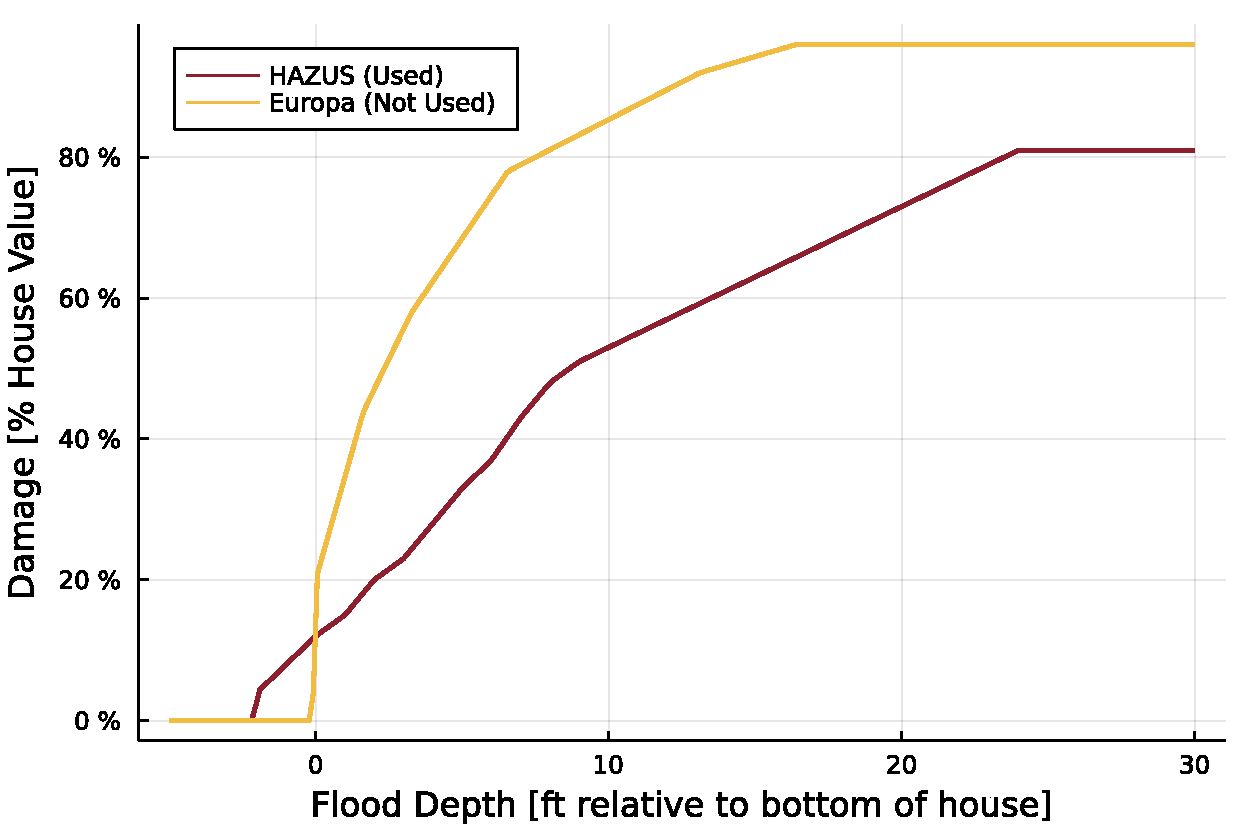
\includegraphics[width=4in]{cost-depth-damage}
      \caption{
            Depth-damage relationship.
            Following \citeA{zarekarizi_suboptimal:2020}, we use the \gls{hazus} depth-damage curves.
            Since results are sensitive to choice of depth-damage equation, we illustrate (for comparison only) the ``Europa'' depth-damage relationship developed by the Joint Research Center (JRC) of the European Commission's science and knowledge service \cite{huizinga_depthdamage:2016}.
      }\label{fig:cost-depth-damage}
\end{figure}

\begin{figure}
      \centering
      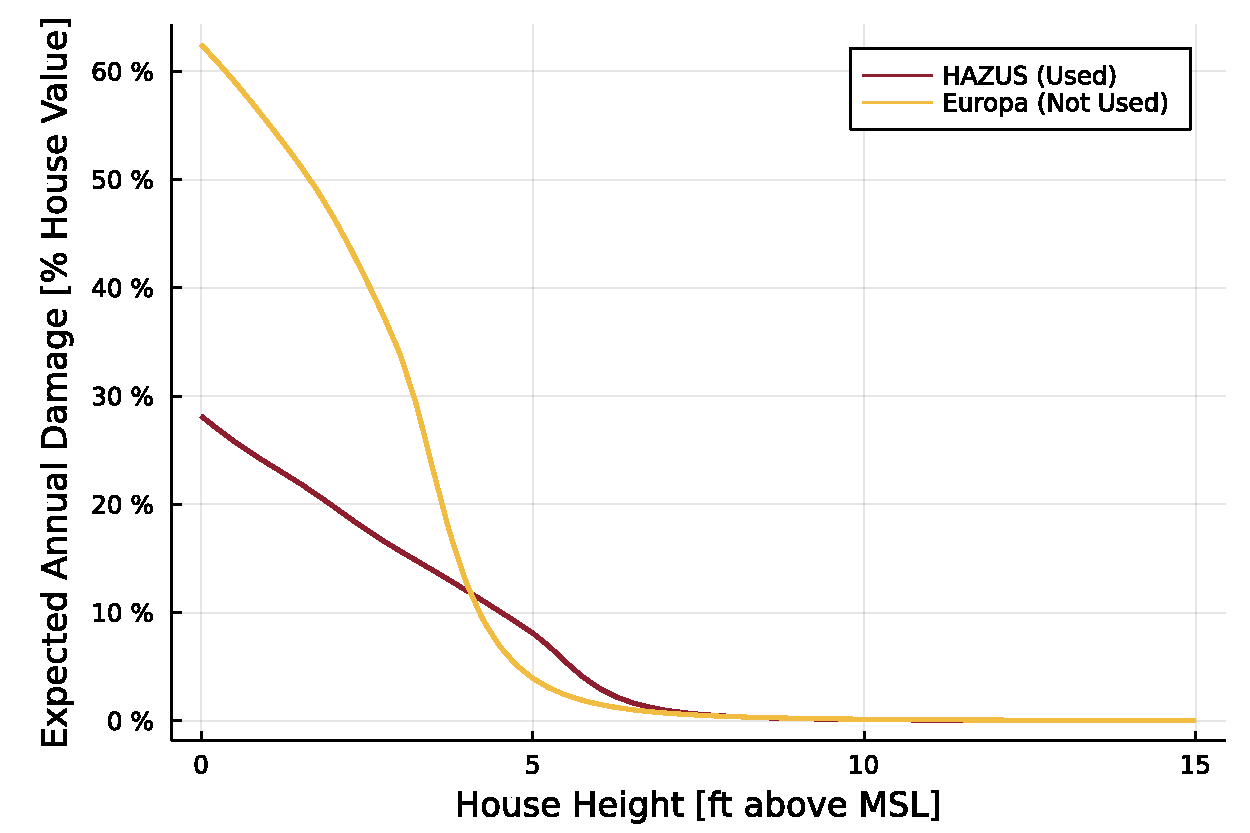
\includegraphics[width=4in]{cost-expected-damage-emulator}
      \caption{
            As discussed in \cref{sec:case-metrics}, we model expected annual damages (eq.~\ref{eq:ead}) as a function of the house's elevation relative to \gls{msl}.
            Damages ($y$ axis) are shown as a percentage of house value.
      }\label{fig:cost-expected-damage-emulator}
\end{figure}

\begin{figure}
      \centering
      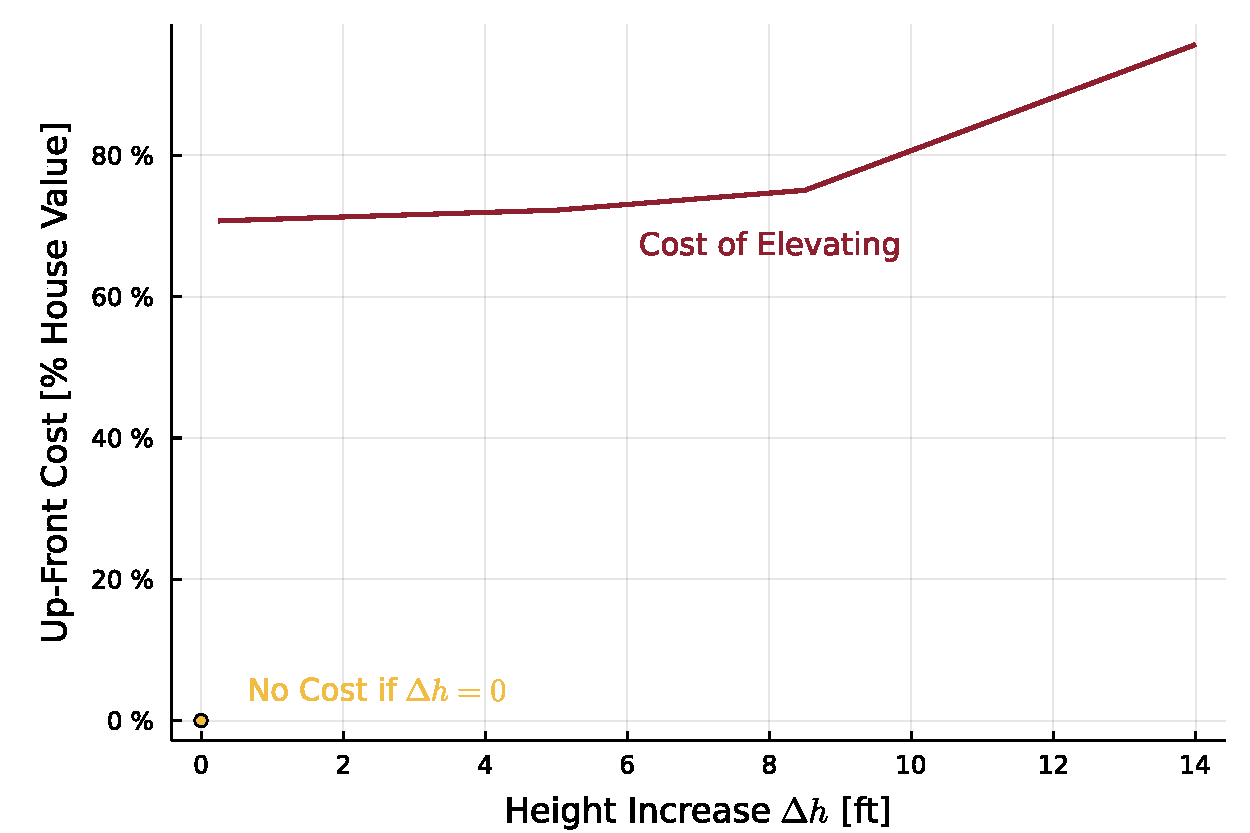
\includegraphics[width=4in]{cost-up-front}
      \caption{
            Following \citeA{zarekarizi_suboptimal:2020}, we model the cost of elevating a single-family house by interpolating estimates from the Coastal Louisiana Risk Assessment Model \cite{johnson_clara:2013}.
            According to this model, the unit cost of elevating a house by 3-7, 7-10, and 10-14 feet is \usd{82.50}, \usd{86.25}, and \usd{103.75} per square foot, respectively, with a \usd{20745} initial cost.
            Values are sensitive to house floor area and structural value; see \cref{tab:uncertainties}.
      }\label{fig:cost-up-front}
\end{figure}

\begin{figure}
      \centering
      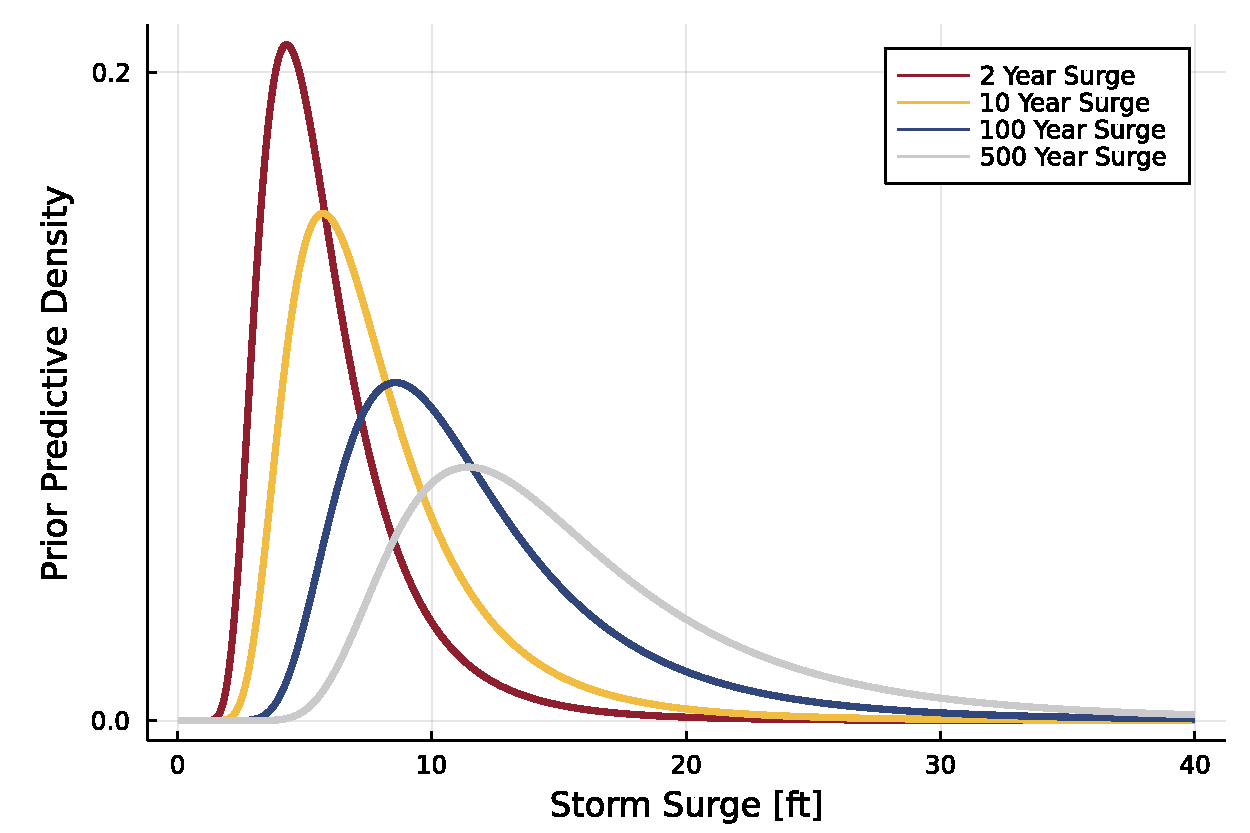
\includegraphics[width=4in]{surge-gev-priors}
      \caption{
            Prior distributions for annual maximum storm surge.
            Rather than apply a prior over model parameters directly, we apply a weakly informative prior over quantiles of the resulting distribution (that is, over a function of the model parameters) following \citeA{coles_evd:1996}.
            See \cref{sec:case-surge} for details.
            For the 2, 10, 100, and 500 year events we apply Inverse Gamma distributions, with means \SIlist{4;6;10;15}{ft} and standard deviations \SIlist{1.5;1.75;2.25;2.75}{ft}, respectively.
      }\label{fig:surge-gev-priors}
\end{figure}

\begin{figure}
      \centering
      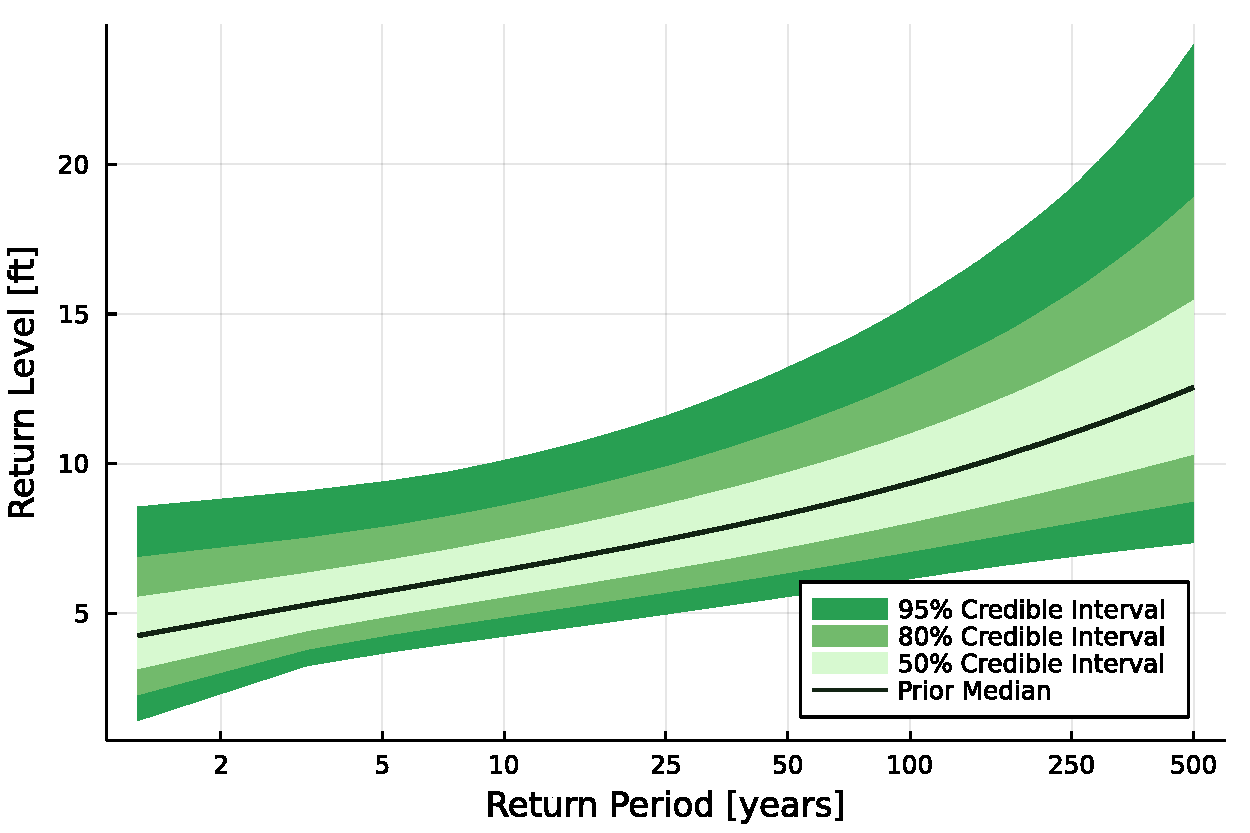
\includegraphics[width=\textwidth]{surge-prior-return}
      \caption{
            Implicit prior over storm surge represents large uncertainty but is consistent with basic physical reasoning (see \cref{sec:case-surge}).
            The prior median (blue line) and uncertainty quantiles (shading) of the return period for different return levels of storm surge at Sewells Point, VA using prior predictive sampling \cite{gelman_workflow:2020}.
            This illustrates the weakly informative prior information (\cref{sec:case-surge}) used in the analysis.
            These weakly informative priors were selected to be consistent with basic physical principles (\eg, storm surges most years are $>$ \SI{2}{ft} but rarely exceed \SI{20}{ft}).
      }\label{fig:surge-prior-return}
\end{figure}

\begin{figure}
      \centering
      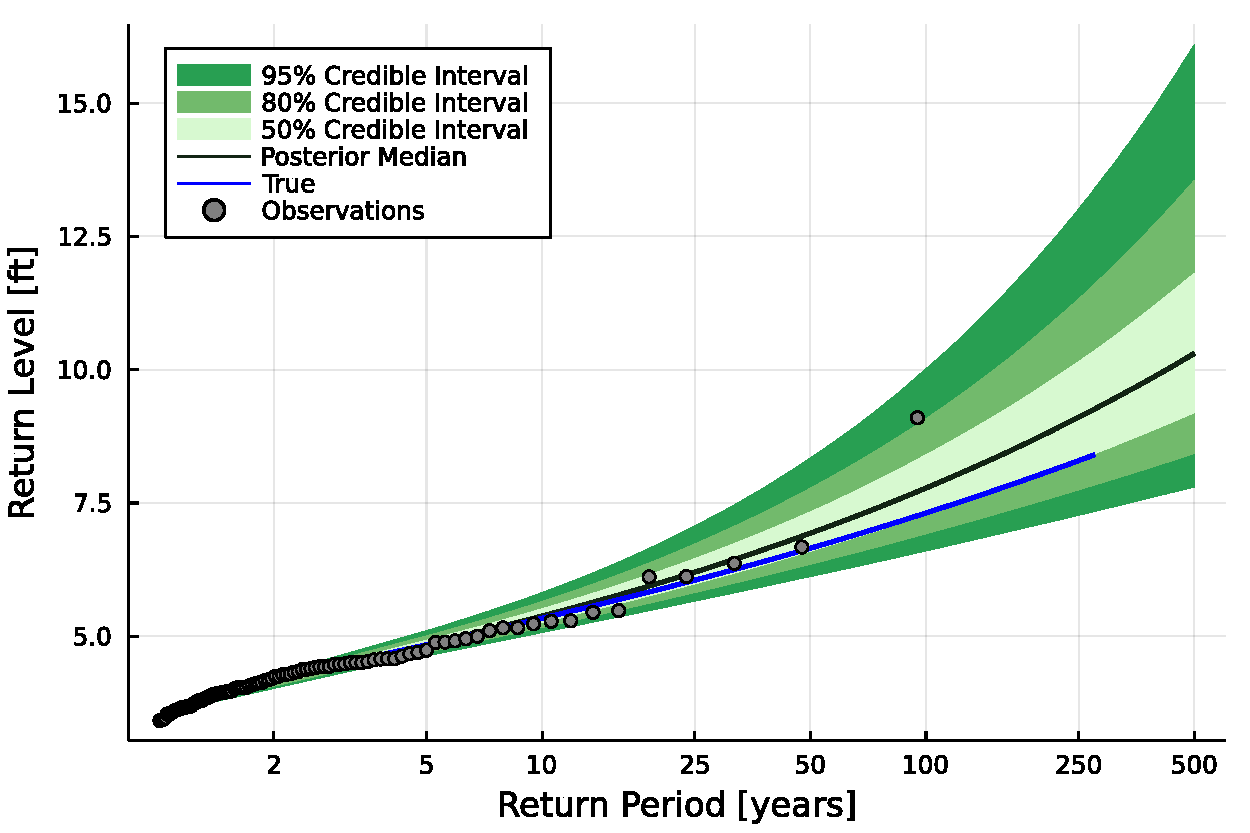
\includegraphics[width=\textwidth]{surge-synthetic-data-experiment}
      \caption{
            Synthetic data experiment as a positive control test for the \gls{gev} model of storm surge.
            A synthetic record (dots) was sampled from a \gls{gev} distribution with location, scale, and shape parameters of 4, 0.5, and 0.15, respectively.
            These samples were used to fit the Bayesian \gls{gev} model described in \cref{sec:case-surge}; the gray shading indicates the 50, 80, and 95\% posterior confidence intervals.
            The blue line shows the true quantiles of the (known) \gls{gev} distribution.
            By random chance the sample maximum has a true return period of $\gg 250$ years, which increases the upper confidence interval of the estimated return probabilities, but the true value is nevertheless within the 50\% posterior confidence interval.
            This experiment yields similar results for alternative values of the known \gls{gev} distribution, and for different random seeds (not shown).
      }\label{fig:surge-synthetic-data-experiment}
\end{figure}

\begin{figure}
      \centering
      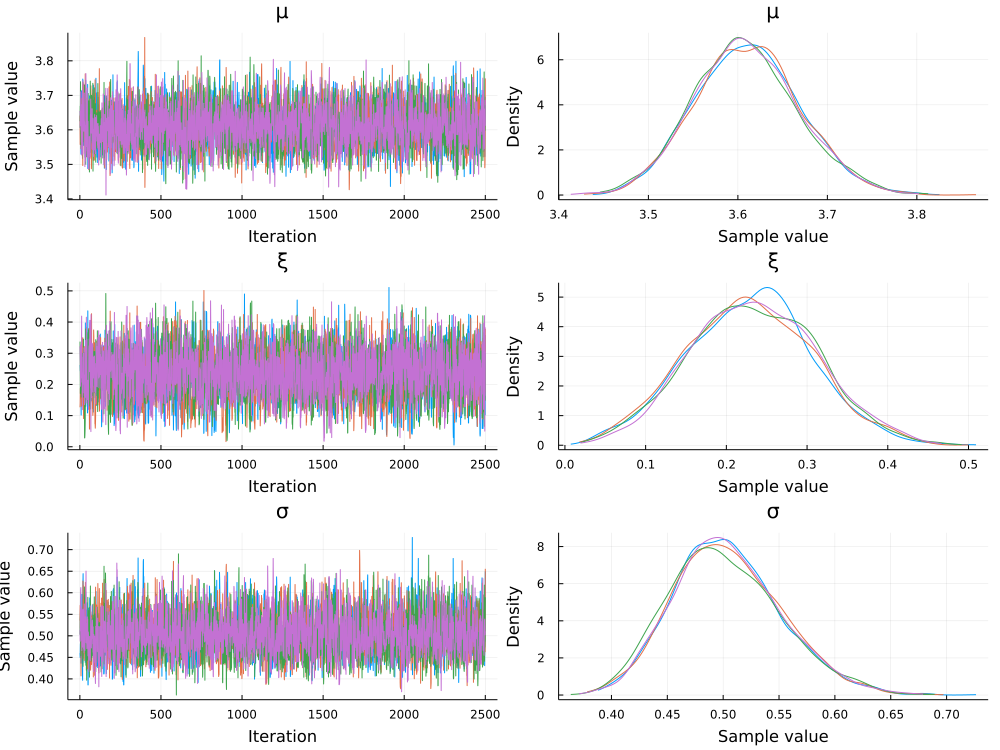
\includegraphics[width=\textwidth]{surge-posterior-chains}
      \caption{
            Markov chain diagnostic plots for posterior draws from the storm surge model.
            We draw \num{10000} samples by running four chains of \num{3500} iterations each and discarding the first \num{1000}.
            The mixing of the chains is consistent with, though does not guarantee, convergence.
      }\label{fig:surge-posterior-chains}
\end{figure}

\begin{figure}
      \centering
      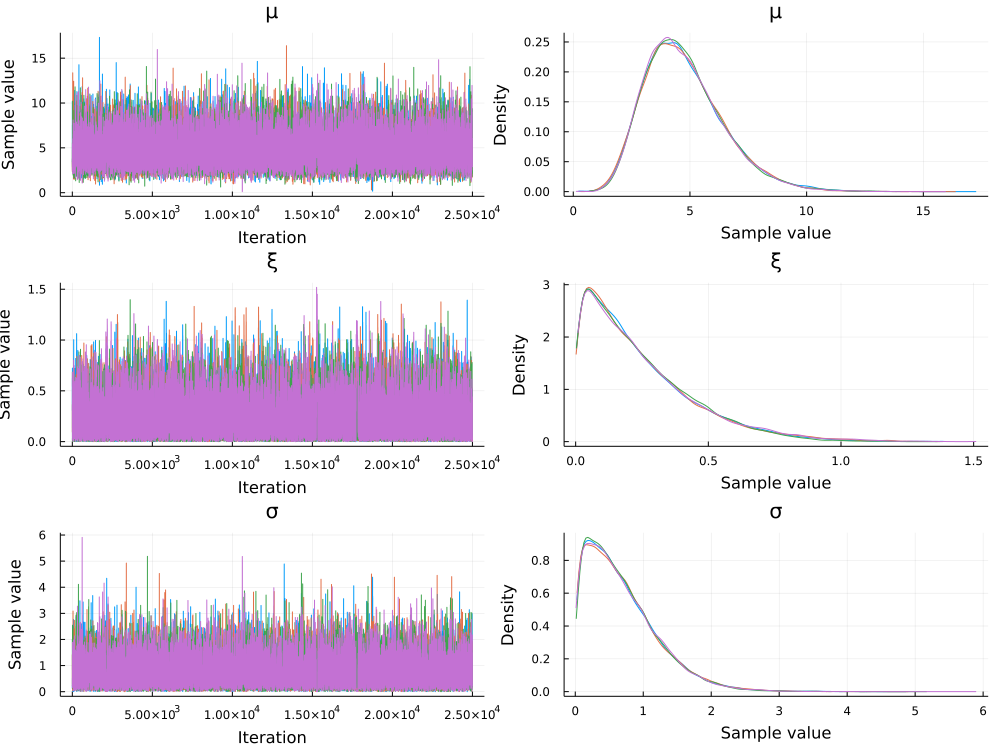
\includegraphics[width=\textwidth]{surge-prior-chains}
      \caption{
            As \cref{fig:surge-posterior-chains}, but for draws from the prior distribution.
      }\label{fig:surge-prior-chains}
\end{figure}

\begin{figure}
      \centering
      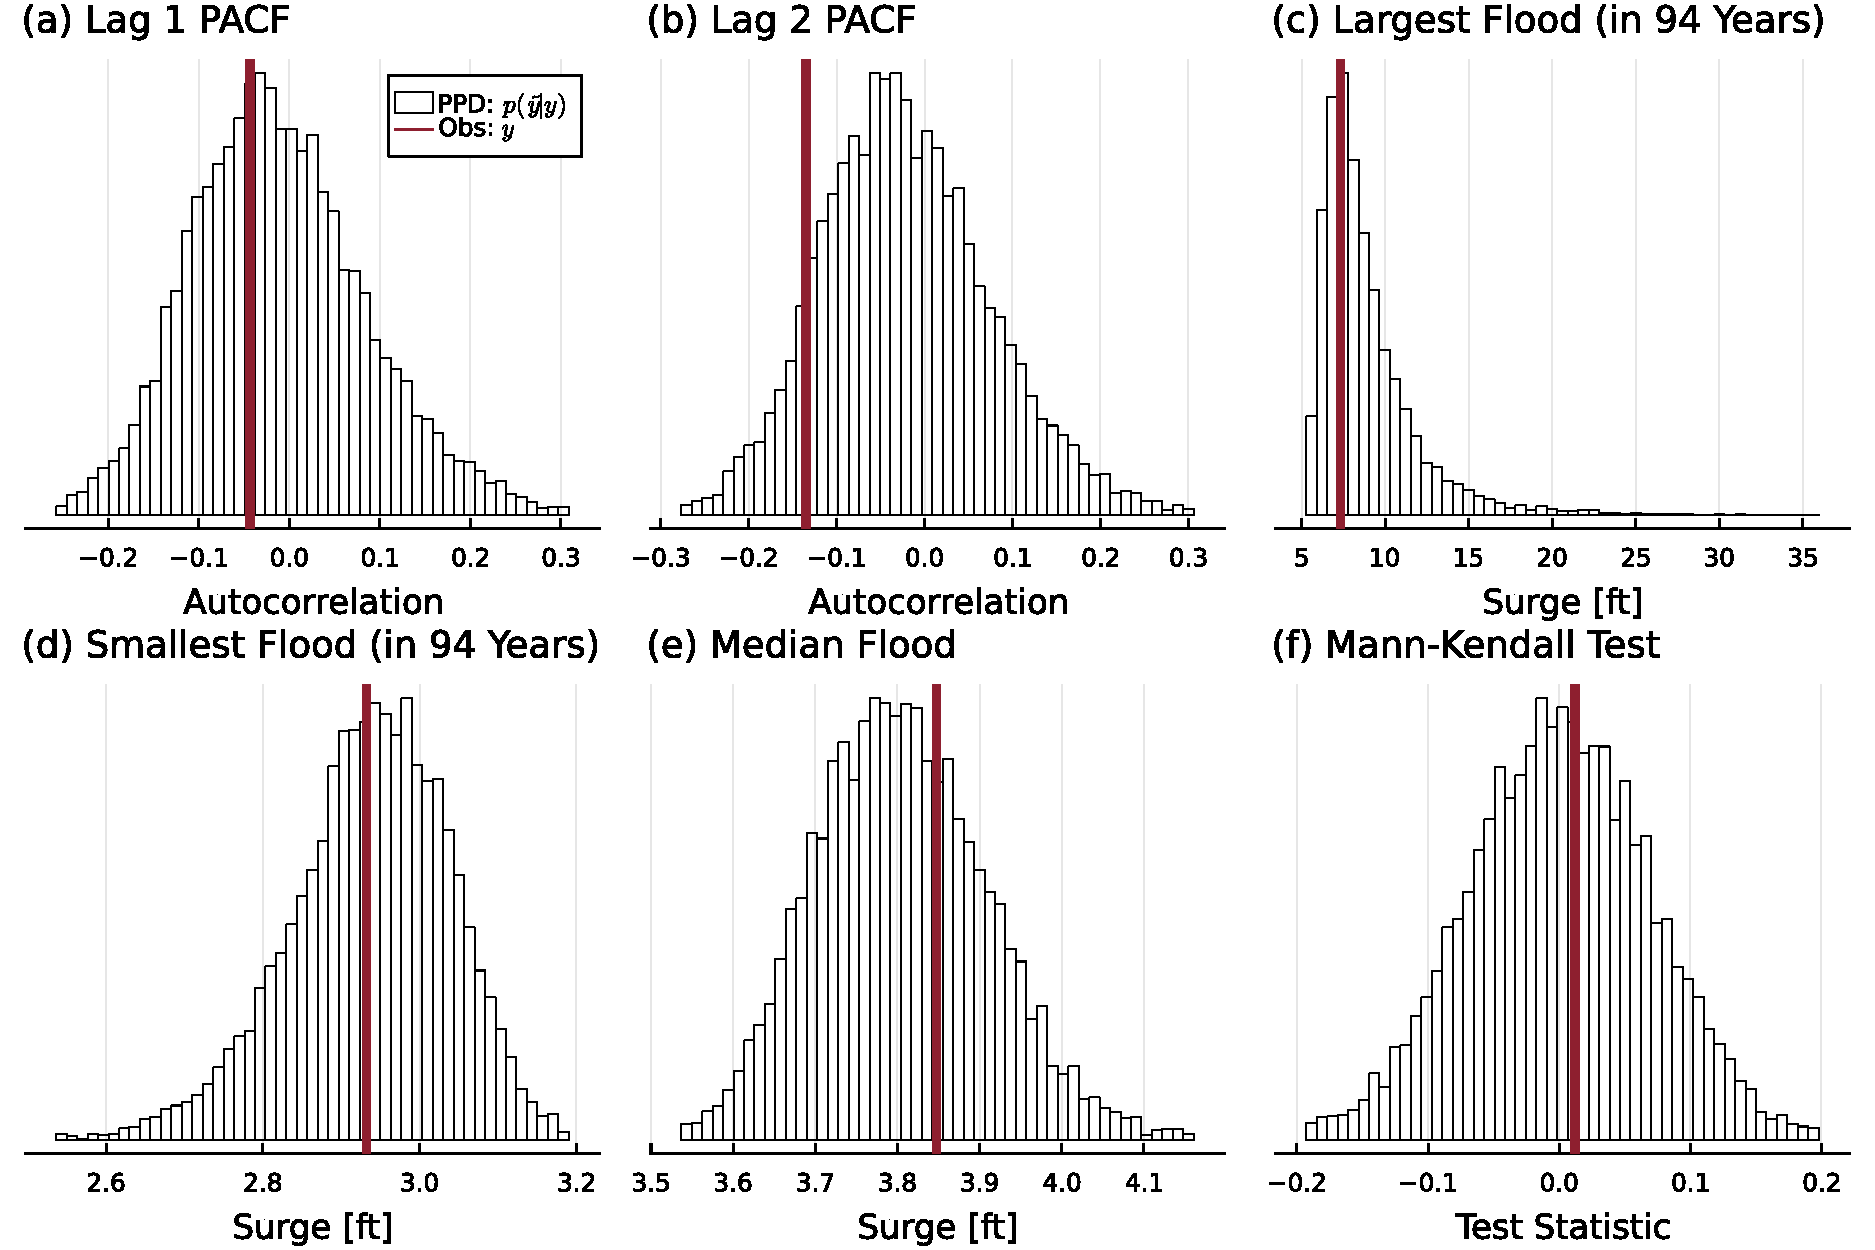
\includegraphics[width=\textwidth]{surge-test-statistics}
      \caption{
            Posterior predictive checks for the stationary \gls{gev} storm surge model (\cref{sec:case-surge}).
            Each panel shows a different test statistic: partial autocorrelation at lags 1 and 2; sample maximum; sample minimum; sample median; and Mann-Kendall trend test statistic.
            The histograms show the distribution of each test statistic from the posterior predictive distribution.
            Orange lines show the test statistic's value in the observed data.
            Observed values near the mode of the posterior predictive distribution are consistent with, but do not guarantee, a good fit.
            For further discussion of posterior predictive checks, see Chapter 6 of \citeA{gelman_bda3:2014}.
      }\label{fig:surge-test-statistics}
\end{figure}

\begin{figure}
      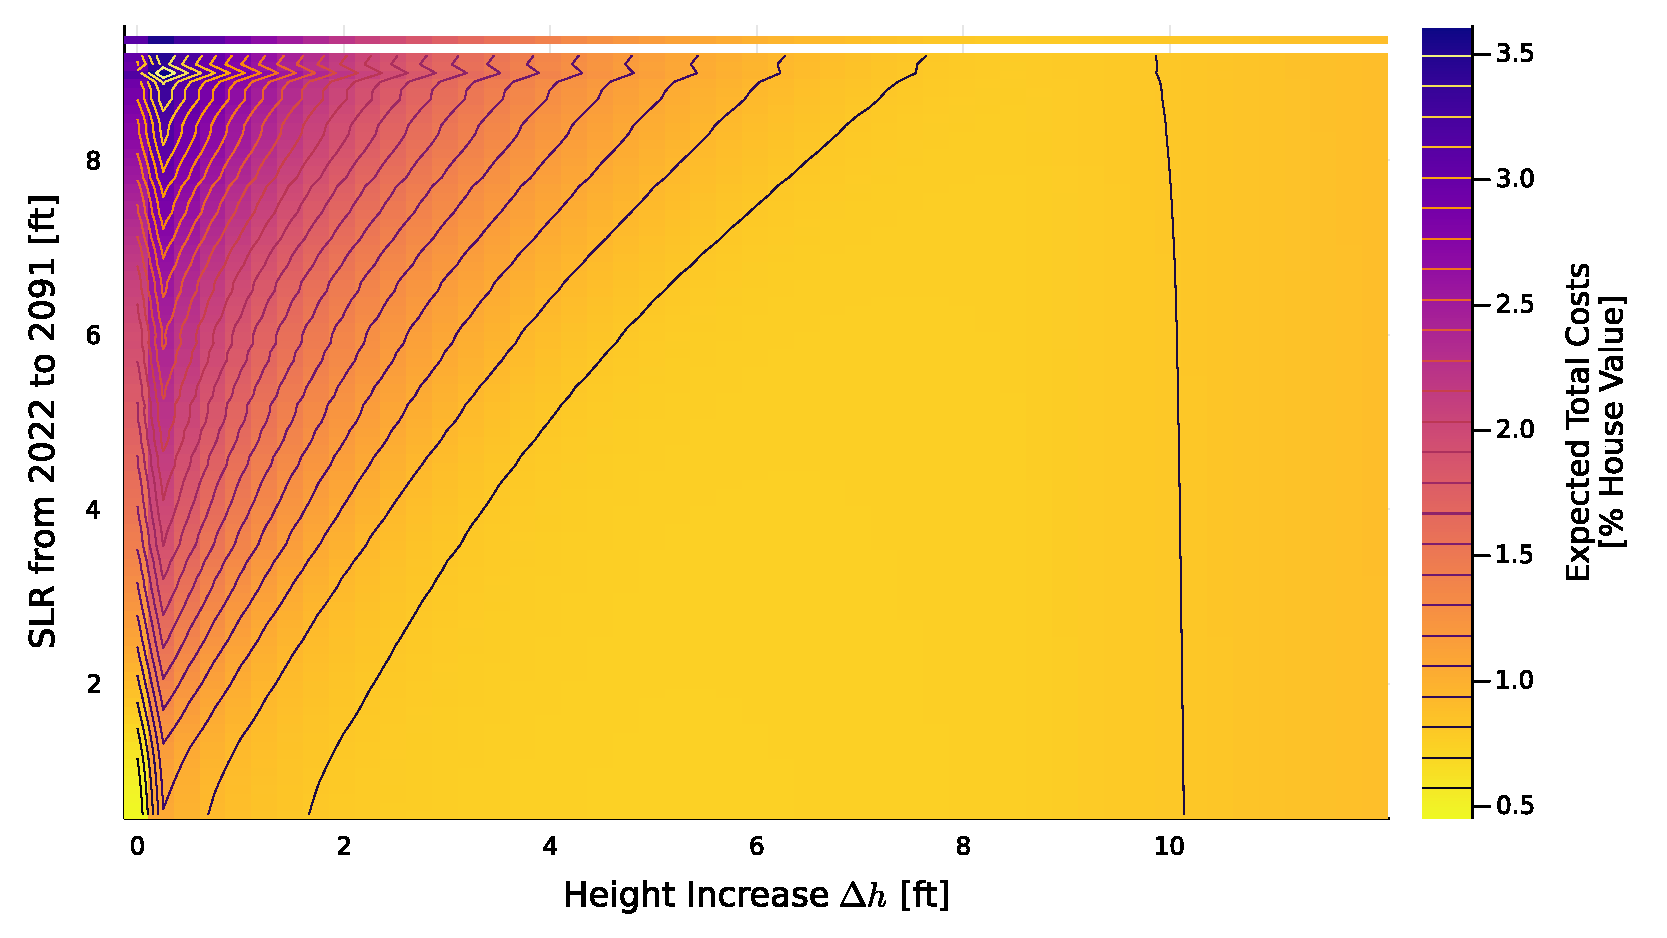
\includegraphics[width=\textwidth]{scenario-map-height-slr}
      \caption{
            Expected total lifetime cost (damages plus up-front cost) as a function of \gls{slr} over the house lifetime and height increase $\Delta h$.
            Initial house elevation is fixed to \SI{1}{ft} below the \gls{bfe}.
            Expectations were computed for discrete values of $\Delta h$ ($x$ axis) by discretizing \glspl{sow} ($y$ axis), then taking the sample mean over each grid cell.
      }\label{fig:scenario-map-height-slr}
\end{figure}

\begin{table}[h]
      \centering
      \caption{
            Diagnostic statistics for the Hamiltonian Monte Carlo sampling for the storm surge posterior draws.
            Statistics include the mean and standard deviation of each parameter, the naive standard error and Monte Carlo standard error (which measure uncertainty in the mean), the effective sample size, $\hat{R}$ diagnostic, and effective samples per second, which describes sampling speed.
            The naive standard error (SE) returns the standard error of the mean.
            The Monte Carlo standard error (MCSE) is calculated using the initial monotone sequence estimator \cite[pp.~473-483]{geyer_practical:1992}.
            The effective sample size (ESS) is a crude estimate of the number of independent samples and is calculated following \citeA[pp.~473-483]{geyer_practical:1992}.
            The $\hat{R}$ is an indicator of the convergence of the Markov chains to the target distribution; a value $\hat{R}$ value close to one is consistent with, though does not guarantee, convergence \cite{mcelreath_rethinking2:2020}.
            For additional details see the \texttt{MCMCDiagnosticTools} package documentation.
      }\label{tab:surge-posterior-mcmc-diagnostics}
      \begin{tabular}{ccccccc}
            \toprule
            $\textrm{Parameter}$ & $\textrm{Mean}$ & $\textrm{Stdev.}$ & $\textrm{Naive SE}$ & $\textrm{MCSE}$ & $\textrm{ESS}$ & $\hat{R}$ \\
            \midrule
            $\mu$                & $3.610$         & $0.059$           & $0.001$             & $0.001$         & $4922.462$     & $1.001$   \\
            $\xi$                & $0.231$         & $0.079$           & $0.001$             & $0.001$         & $4609.415$     & $1.001$   \\
            $\sigma$             & $0.504$         & $0.049$           & $0.000$             & $0.001$         & $4547.881$     & $1.001$   \\
            \bottomrule
      \end{tabular}

\end{table}

\begin{table}[h]
      \centering
      \caption{As \cref{tab:surge-posterior-mcmc-diagnostics} but for draws from the prior distribution.}\label{tab:surge-prior-mcmc-diagnostics}
      \begin{tabular}{ccccccc}
            \toprule
            $\textrm{Parameter}$ & $\textrm{Mean}$ & $\textrm{Stdev.}$ & $\textrm{Naive SE}$ & $\textrm{MCSE}$ & $\textrm{ESS}$ & $\hat{R}$ \\
            \midrule
            $\mu$                & $4.774$         & $1.702$           & $0.005$             & $0.011$         & $26657.405$    & $1.000$   \\
            $\xi$                & $0.246$         & $0.215$           & $0.001$             & $0.002$         & $11238.145$    & $1.000$   \\
            $\sigma$             & $0.682$         & $0.531$           & $0.002$             & $0.004$         & $24720.263$    & $1.000$   \\
            \bottomrule
      \end{tabular}

\end{table}


\end{document}

